% MACHETE:


%    --- Enfatizar "con hipotesis de que solo pasan al final una vez y llenan dames, se puede visualizar con bastante éxito que reglas chinas/de area
%         como que también están contando territorio y al final redondean de acuerdo a la paridad de los seki-dames.
%    --- Las otras diferencias que no son realmente necesarias en conteo área / conteo territorio pasa por qué cosas consideramos territorio o no.
    
    



\documentclass{beamer}

\mode<presentation>
{
  \usetheme{Warsaw}
  \useoutertheme{infolines}
  % or ...

  \setbeamercovered{transparent}
  % or whatever (possibly just delete it)
}

\usepackage{multicol}
\usepackage{graphicx}
\usepackage{wrapfig}
\usepackage{verbatim}
\usepackage{amsmath}
\usepackage{listings}
\usepackage{ulem}

\lstloadlanguages{C++}
\lstnewenvironment{code}
	{%\lstset{	numbers=none, frame=lines, basicstyle=\small\ttfamily, }%
	 \csname lst@SetFirstLabel\endcsname}
	{\csname lst@SaveFirstLabel\endcsname}
\lstset{% general command to set parameter(s)
	language=C++, basicstyle=\footnotesize\sffamily, keywordstyle=\slshape,
	emph=[1]{tipo,usa}, emphstyle={[1]\sffamily\bfseries},
	morekeywords={tint,forn,forsn},
	basewidth={0.47em,0.40em},
	columns=fixed, fontadjust, resetmargins, xrightmargin=5pt, xleftmargin=15pt,
	flexiblecolumns=false, tabsize=2, breaklines,	breakatwhitespace=false, extendedchars=true,
	numbers=left, numberstyle=\tiny, stepnumber=1, numbersep=9pt,
	frame=l, framesep=3pt,
}

\usepackage[spanish]{babel}
% or whatever

\usepackage[utf8]{inputenc}
% or whatever

\usepackage{times}
\usepackage[T1]{fontenc}
% Or whatever. Note that the encoding and the font should match. If T1
% does not look nice, try deleting the line with the fontenc.


\title % (optional, use only with long paper titles)
{Reglas Fantásticas y dónde encontrarlas}

\author[Agustín Gutiérrez] % (optional, use only with lots of authors)
{~Agustín Santiago Gutiérrez}

% - Give the names in the same order as the appear in the paper.
% - Use the \inst{?} command only if the authors have different
%   affiliation.
\institute[AAGO] % (optional, but mostly needed)
{
  Asociación Argentina de GO
}
\date[Congreso 2021] % (optional, should be abbreviation of conference name)
{Congreso Argentino de Go 2021}

% Acá se puede insertar el logo de la UBA
% \pgfdeclareimage[height=0.5cm]{university-logo}{university-logo-filename}
% \logo{\pgfuseimage{university-logo}}

% Delete this, if you do not want the table of contents to pop up at
% the beginning of each subsection:
\AtBeginSection[]
{
  \begin{frame}{Contenidos}
  \footnotesize
    \tableofcontents[currentsection, currentsubsection]
  \end{frame}
}

% If you wish to uncover everything in a step-wise fashion, uncomment
% the following command: 

%\beamerdefaultoverlayspecification{<+->}


\begin{document}

\begin{frame}
  \titlepage
\end{frame}

\begin{frame}{Contenidos}
  \footnotesize
  \tableofcontents
  % You might wish to add the option [pausesections]
\end{frame}

\begin{frame}
  Una excepción no es más que una regla que aplica excepcionalmente.
  
  
  \ 
  
  \hfill \ \ \ \ \ \ \ \ \textit{Fausto Cercignani}

  \ 
  
  \ 
  
  \  
  
  Conoce bien las reglas, para poder romperlas con efectividad.
  
  \ 
  
  \hfill \ \ \ \ \ \ \ \ Falsamente atribuida al \textit{Dalai Lama} en internet
  
  \ 
  
  \ 
  
  \ 

  Si una regla evita que mejores o mantengas Wikipedia, ignórala.

  \ 
  
  \hfill \ \ \ \ \ \ \ \ \textit{Wikipedia:Ignore\_all\_rules}
\end{frame}


\section{Preliminar}

\begin{frame}{Aclaraciones y suposiciones}
  Aclaraciones:
  
  \begin{itemize}
  \item Hay \textbf{demasiado} material para cubrir en solo una hora
  \item La utilidad de esta charla para subir de categoría es despreciable
  \item Existen las \textit{reglas de juego} y las \textit{reglas de torneo}. 
  \item La charla focaliza únicamente sobre las reglas de juego
  \end{itemize}
  
  Suposiciones:
  
  \begin{itemize}
  \item Saben las reglas (``básicas'' o ``normales'') y han jugado varias partidas sin problemas de reglas
  \item Están más familiarizados con conteo de territorio (``japonés'') que de área (``chino'')
  \end{itemize}
  
  
\end{frame}

\section{Historia de las reglas y disputas}

\begin{frame}{Primeras reglas de go}
  
  \begin{itemize}
    \item Se cree que fue primero el \textbf{conteo de piedras} en China
    
    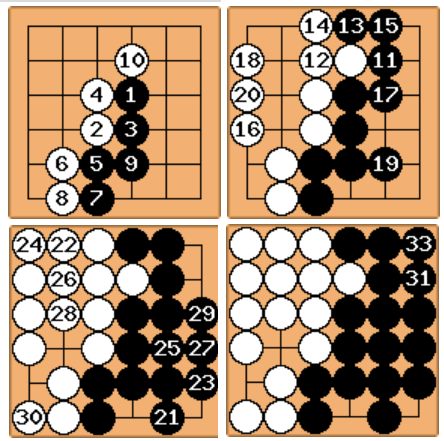
\includegraphics[scale=0.3]{conteopiedraspartida.png}
    
  \end{itemize}
  
\end{frame}

\begin{frame}{Reglas chinas}
  
  \begin{itemize}
    \item Conteo de piedras $\rightarrow$ \textbf{conteo de área}, en China
    \item Evidencia de uso en Dinastía Ming (siglo XV o XVI)
    
    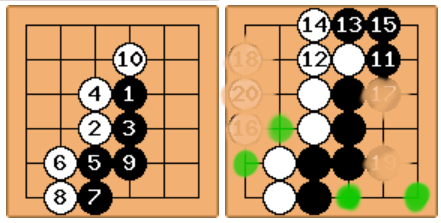
\includegraphics[scale=0.5]{conteoareapartida.png}
    
    \item Los puntos verdes no los hubiera contado el conteo de piedras
  \end{itemize}
  
\end{frame}

\begin{frame}{Reglas japonesas}
  
  \begin{itemize}
    \item China $\rightarrow$ Japón: \textbf{conteo de territorio}
    
    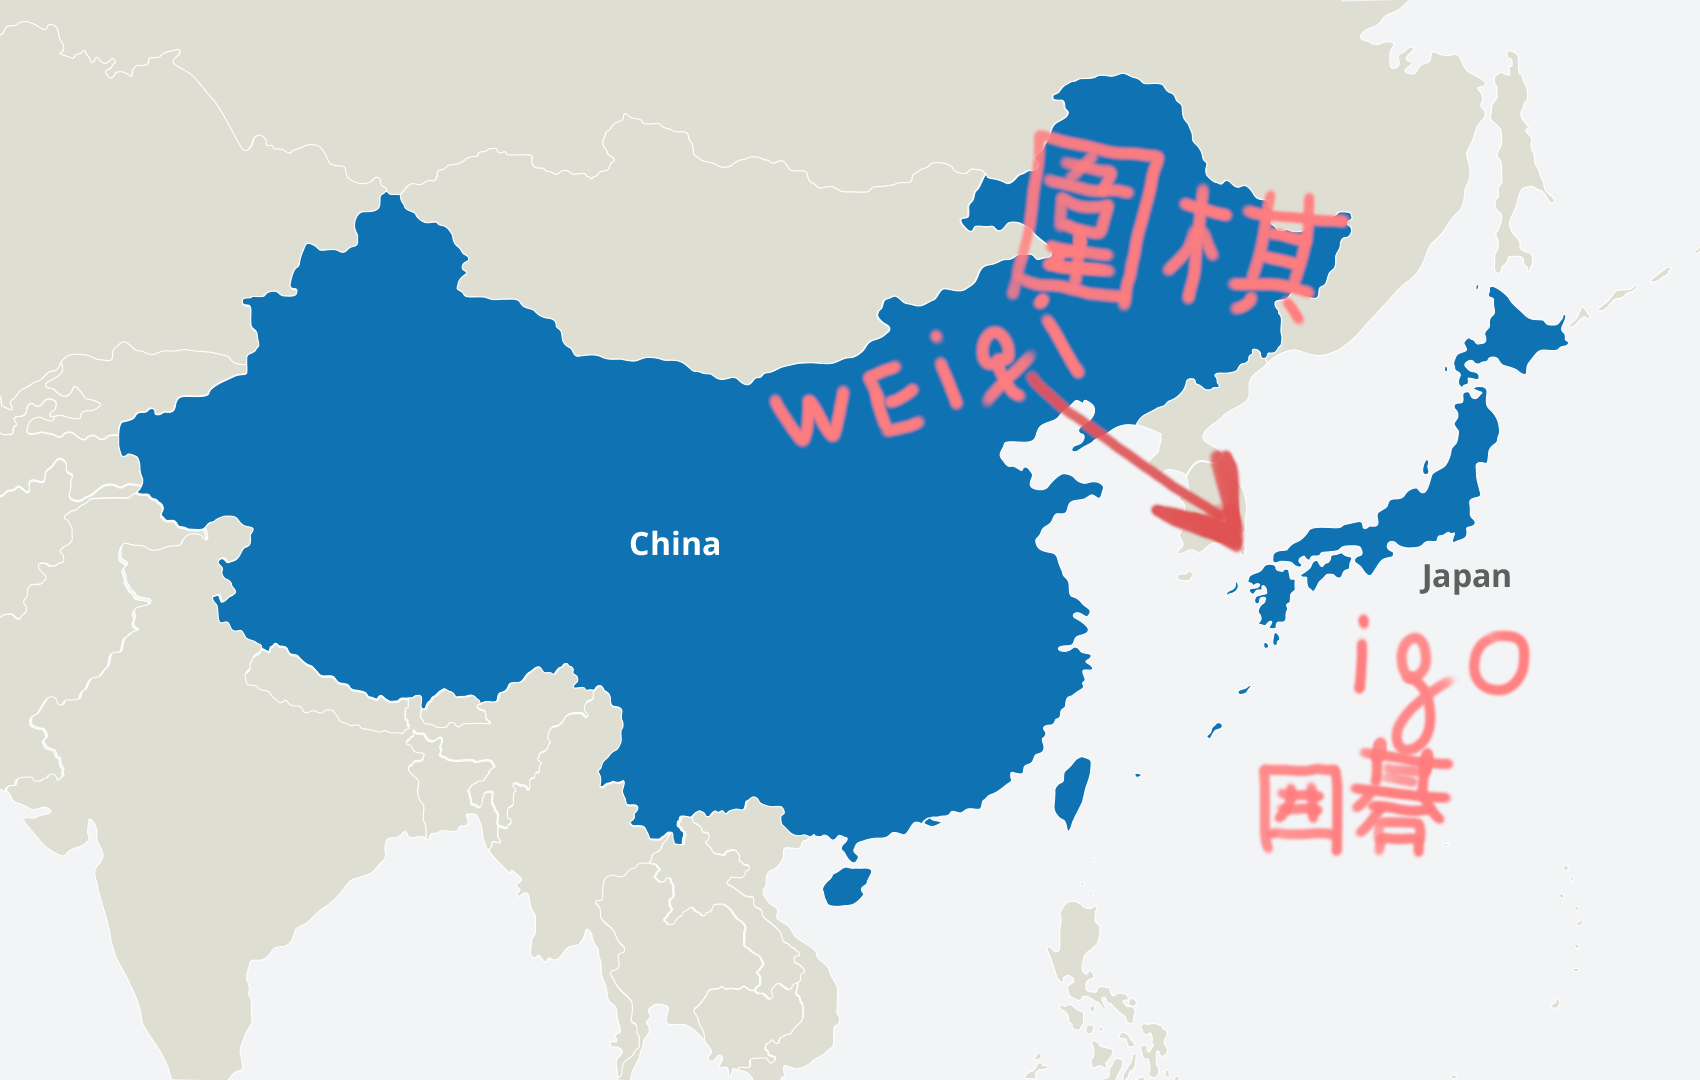
\includegraphics[scale=0.2]{chinajapon.png}
  \end{itemize}
  
\end{frame}


\begin{frame}{Primera disputa de reglas registrada}
  
  \begin{itemize}
    \item 1253: Un caso de \textbf{falsa vida}
    \item ¿Vivo? ¿Muerto?
    \item Fallo final ``polémico'' del monje Nyobutsu
    \item Decide \textbf{al revés que las reglas actuales}
    \item Durante los siglos siguientes, no hubo consenso en Japón
    
  \end{itemize}
  
\end{frame}

\begin{frame}{Crisis de 1928}
  \begin{itemize}
    \item 1928: Segoe Kensaku vs Takahashi Shigeyuki
    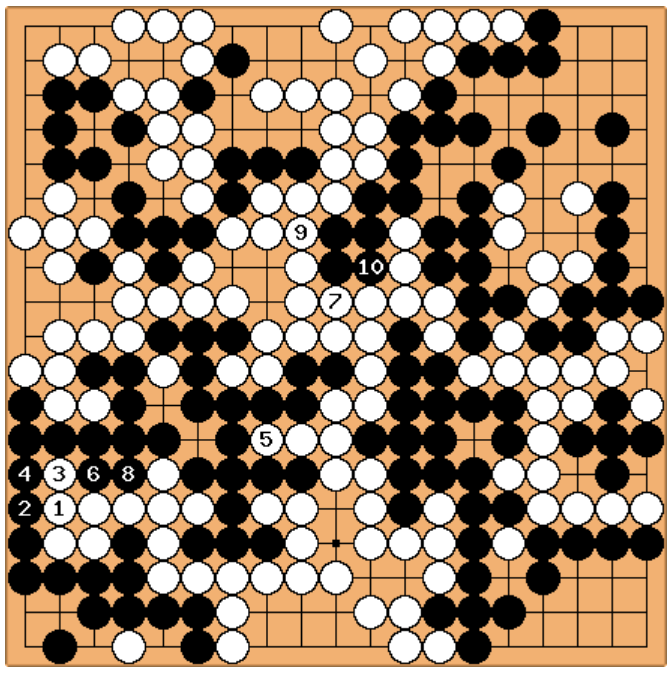
\includegraphics[scale=0.15]{rulecrisis.png}
    \item A la derecha, queda un ko de 10 mil años sin resolver
    \item Precipita extenso debate y crisis de reglas en Japón
    \item Honinbo Shusai y Okura Kishichiro determinan sin explicación: \\
    \ \\
          \ \ \ \ \ \ \ \textbf{``Blanco ganó, pero negro no perdió.''}
  \end{itemize}

\end{frame}

\begin{frame}{Dos disputas de Go Seigen}
  \begin{itemize}
    \item 1948: Go Seigen vs Iwamoto Kaoru.
    \begin{itemize}
    \item Se disputa si hace falta defender el último ko, aún si a blanco le sobran amenazas de ko y no hay dames
    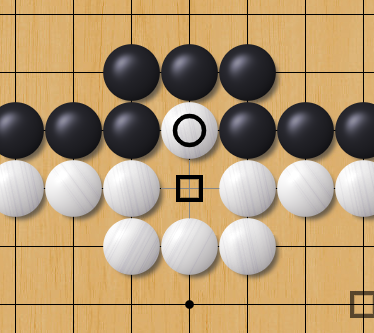
\includegraphics[scale=0.2]{ultiko.png}
    \item No defender permitiría ganar un punto adicional de territorio
    \item Se decide en ese momento (Honinbo Shusai y Go Seigen están de acuerdo) que \textbf{no} hace falta defender el ko
    \item Esto perjudica a Go Seigen en el partido
    \end{itemize}
  \end{itemize}

\end{frame}

\begin{frame}{Dos disputas de Go Seigen (cont.)}
  \begin{itemize}
    \item 1959: Go Seigen vs Takagawa Shukaku.
    \begin{itemize}
    \item Se da la misma situación.
    \item Esta vez el punto extra sería para Go Seigen.
    \item Tras meses de disputa, esta vez se decide que \textbf{sí} es obligación defender el ko.
    \item Go Seigen pierde por medio punto.
    \end{itemize}
  \end{itemize}

\end{frame}



\begin{frame}{Primeras reglas escritas en Japón}
  
  \begin{itemize}
    \item Antes de 1949: no había reglas escritas ``oficiales''. 
       \begin{itemize}
         \item Las disputas eran resueltas por las autoridades
         \item Ejemplo: Honinbo Shuwa y la situación ``Torazu Sanmoku''
       \end{itemize}
    \item Reglas 1949:
    \begin{itemize}
        \item \textbf{Muchos} ``casos especiales'' (``bent four in the corner is dead'')
        \item Si surgen nuevos casos complicados, ``la Nihon Ki-in resolverá''
    \end{itemize}
    \item ``WAGC 1979 Rules'': son más simples, pero también incompletas y con casos especiales. 
    \item Reglas 1989 [\textbf{Reglas japonesas actuales}]:
     \begin{itemize}
        \item Dan un procedimiento general (complicado de formalizar, pero posible) de ``juego hipotético''.
        \item Un grupo está vivo o muerto, según el ``juego hipotético''.
        \item Coincide con casi todos los ejemplos particulares de 1949.
     \end{itemize} 
    
  \end{itemize}
  
\end{frame}

%\begin{frame}{Jugada ilegal de Cho Chikun}
%  
%  \begin{itemize}
%    \item 1980: final del quinto Meijin, Otake Hideo vs Cho Chikun.
%    \item Cho Chikun recaptura un ko inmediatamente, sin hacer una amenaza.
%    \item Por reglamento, pierde por jugada ilegal.
%    \item Pero, Cho preguntó al asistente si era su turno de retomar el ko y este dijo que sí.
%    \item Se decide dejar el partido sin resultado, y jugarlo otra vez.
%    
%  \end{itemize}
%  
%\end{frame}


%\begin{frame}{Disputa Copa Samsung 2004}
%  
%  \begin{itemize}
%    \item Huang Yi-zhong vs Kim Kang-geun.
%    \item Diferencia cultural: en China se devuelven los prisioneros al cuenco, en Corea y Japón no. 
%    \item Por descuido, Huang devolvió un prisionero a Kim, alterando el conteo.
%    \item La prensa China acusó fuertemente a Kim de tramposo, y el manejo de la KBA de la situación fue calificado de ``dudoso''. 
%    
%  \end{itemize}
%  
%\end{frame}

\section{Conteo}

\begin{frame}{Conteo de piedras}
  
  \begin{itemize}
    \item Uno de los más fáciles.
    \item Al terminar, el puntaje es la cantidad de piedras en el tablero. 
    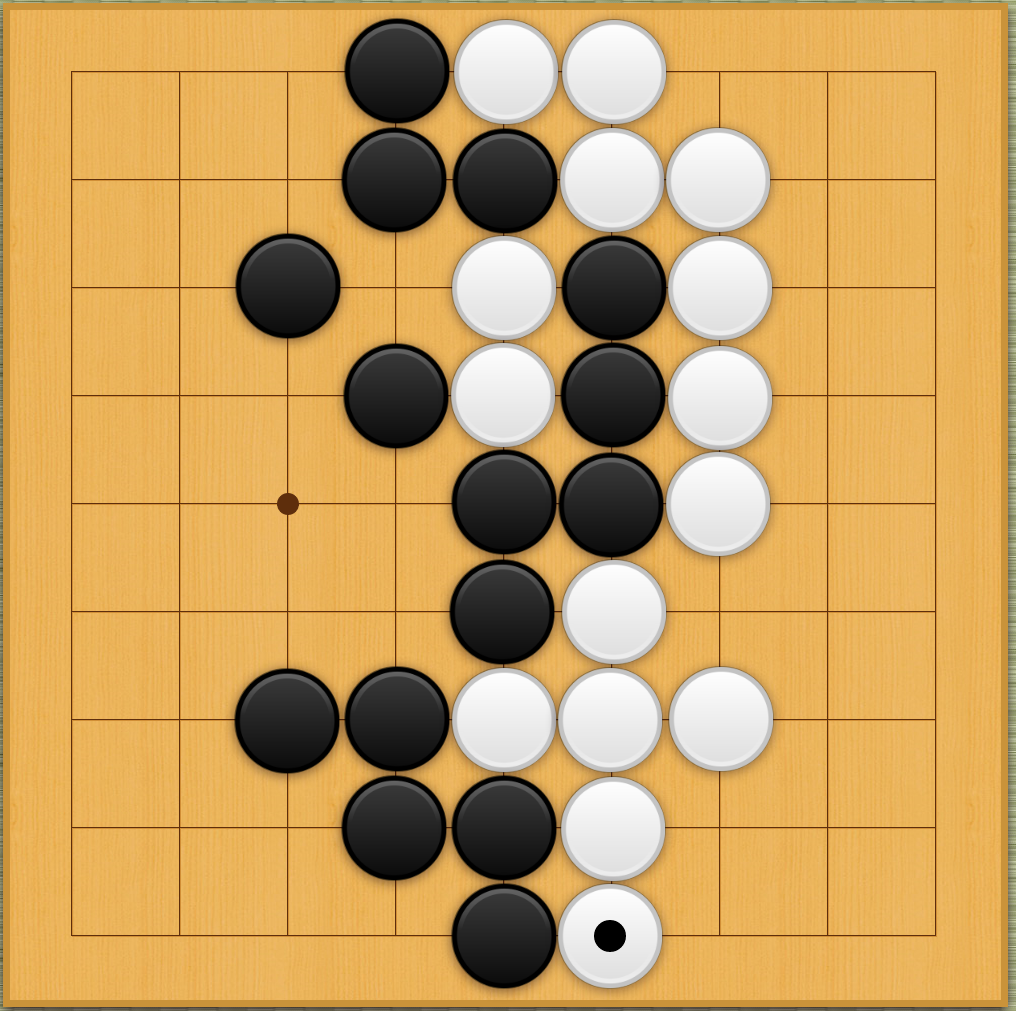
\includegraphics[scale=0.17]{ejemplo-conteo.png} \ \ \ Blanco: 15 \ \ \ Negro : 15  
  \end{itemize}
  
\end{frame}

\begin{frame}{Conteo de piedras (finalizado)}
  
  \begin{itemize}
    \item Por supuesto, a los jugadores les conviene capturar y llenar todo.
    \item El conteo se realiza sobre esa posición.
    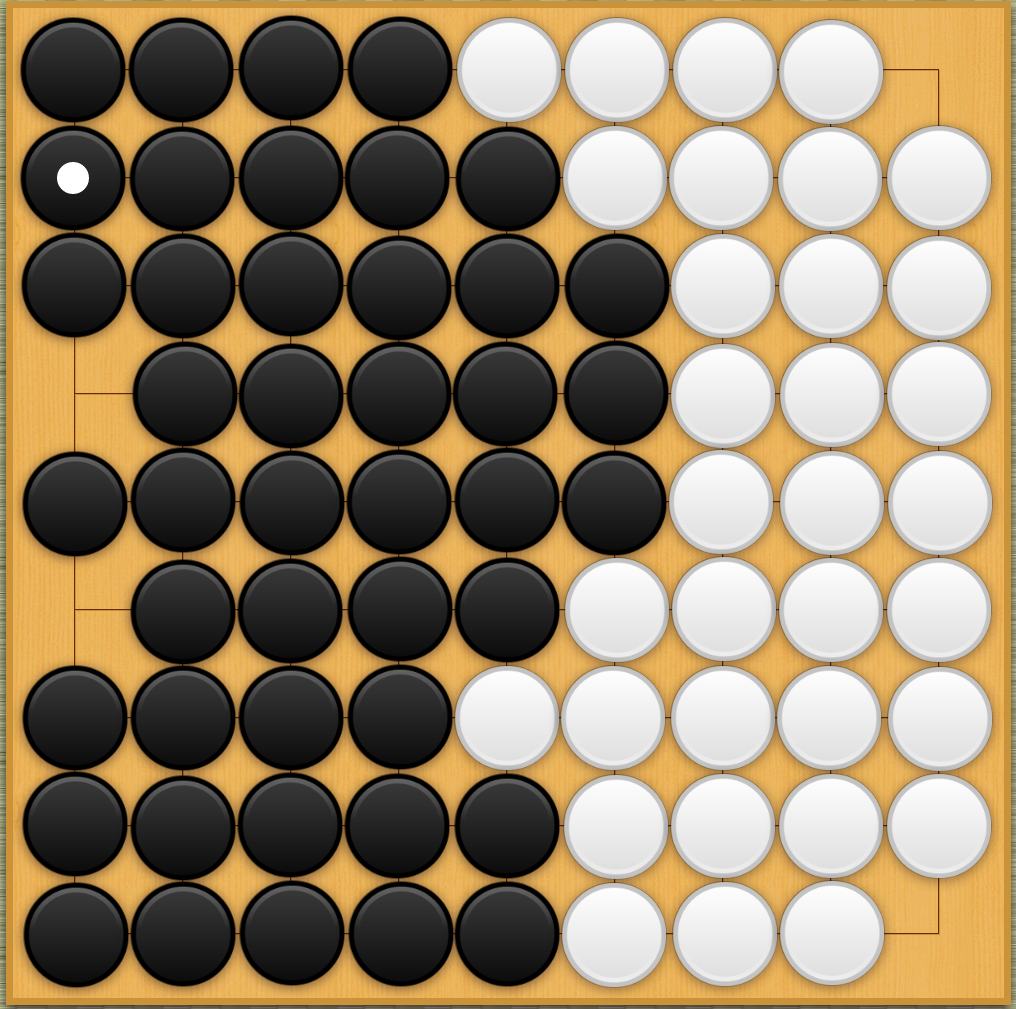
\includegraphics[scale=0.17]{conteo-piedras.png} \ \ \ Blanco: 33 \ \ \ Negro : 44  
  \end{itemize}
  
\end{frame}

\begin{frame}{Conteo de área}
  
  \begin{itemize}
    \item El conteo anterior ``se pierde'' los ojos de cada grupo.
    \item Contando también esos puntos rodeados, queda\\ {\hfill piedras $+$ territorio $=$ \textbf{área} \hfill}
    
    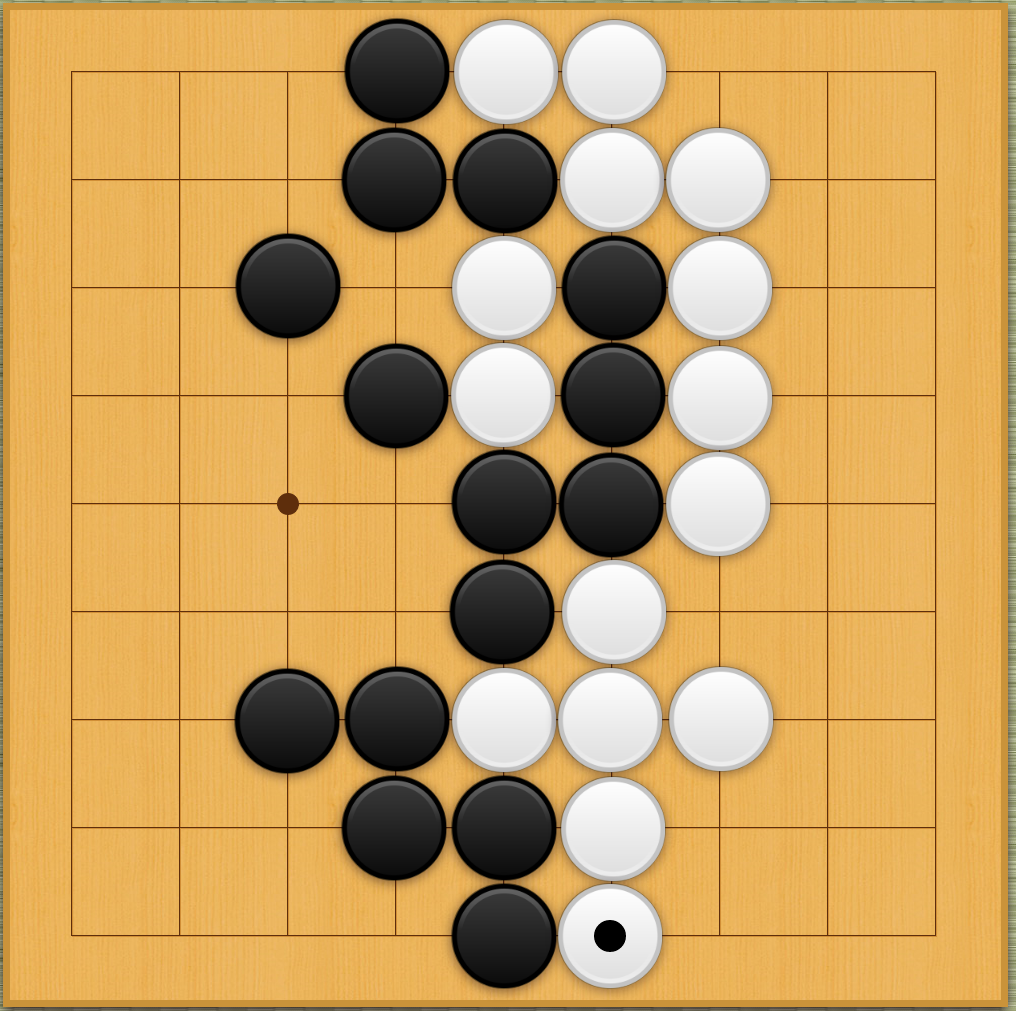
\includegraphics[scale=0.17]{ejemplo-conteo.png} \ \ \ Blanco: 35 \ \ \ Negro : 46  
  \end{itemize}
  
\end{frame}

\begin{frame}{Conteo de área (cont)}
  
  \begin{itemize}
    \item Se usa en las reglas Chinas.
    \item Llenar los territorios propios no tienen ningún valor, pero no resta.
    \item Llenar un dame suma un punto.
    \item Especie de ``Conteo de piedras abreviado'': 
       \begin{itemize}
           \item No hace falta llenar todo de piedras para contar
           \item Alcanza con remover los prisioneros.
       \end{itemize}
    \item \textbf{Si no hay sekis, los puntajes suman 81} (o 361)
    \item \textbf{Si quedan $d$ dames,  los puntajes suman $81 - d$} (o $361 - d$)
    \item Observación: de lo anterior, \textbf{la diferencia de puntajes es siempre impar}, excepto si $d$ es impar (poco frecuente).
  \end{itemize}
  
\end{frame}

\begin{frame}{Conteo de territorio}
  
  \begin{itemize}
    \item Con este sistema, el puntaje es territorio $+$ piedras capturadas.
    
    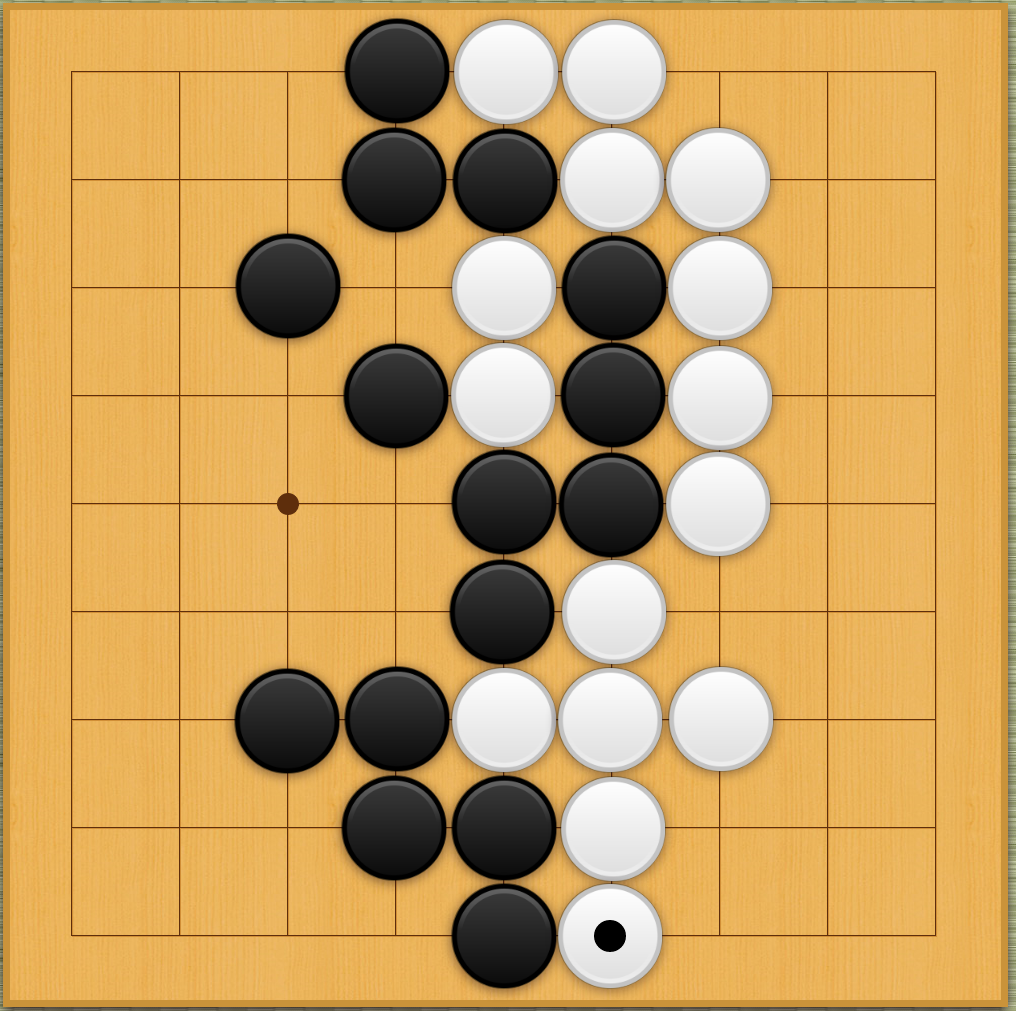
\includegraphics[scale=0.17]{ejemplo-conteo.png} \ \ \ Blanco: 22 \ \ \ Negro : 33  
  \end{itemize}
  
\end{frame}

\begin{frame}{Conteo de territorio (cont)}
  
  \begin{itemize}
    \item Se usa en las reglas Japonesas.
    \item Llenar los territorios propios ahora resta un punto.
    \item Llenar un dame no suma ni resta.
    \item Observación: la diferencia puede ser par o impar, no está restringida como en conteo de área.
  \end{itemize}
  
\end{frame}


\begin{frame}{Conteo territorio = Conteo de área (matemática)}
  
  Con conteo de área:
  \begin{itemize}
    \item En cada jugada ponemos una piedra, así que estamos ``ganando un punto'' por jugada.
    \item Juega una vez cada uno: ¡Esos puntos \textbf{se cancelan}!
    \item La excepción son las capturas: allí un jugador pierde puntos (piedras) pero el otro no.
    \item Solución: no contar las piedras, salvo al ser capturadas, que \textbf{suman puntos al rival}.
    \item Eso es lo que hace el conteo de territorio.
  \end{itemize}
  
  Por esta razón, \textbf{si ambos jugadores jugaron la misma cantidad de veces}, contar área y contar territorio dan exactamente igual diferencia.
  
\end{frame}


\begin{frame}{Conteo territorio = Conteo de área (matemática)}
  
  \begin{itemize}
      \item Si no jugaron la misma cantidad de veces, la diferencia de piedras no se cancela, y como negro jugó una vez más, tiene un punto más con conteo de área. 
  \end{itemize}
  
  \begin{itemize}
      \item Pero la diferencia de conteo de área es impar: por lo tanto, negro tiene ese punto extra en conteo de área, cuando la \textbf{diferencia de territorio} era par.
  \end{itemize}
\end{frame}

\begin{frame}{Conteo territorio = Conteo de área (matemática)}

Lo anterior viene resumido en esta tabla de ejemplo (positivo es que gana negro, negativo que gana blanco):
  
  Si $d$ es par (El caso más habitual: cuando no hay sekis atípicos):
  
  $$\begin{array}{cc}
      \mbox{Diferencia territorio} & \mbox{Diferencia área} \\
      -3 & -3 \\
      -2 & -1 \\
      -1 & -1 \\
      0 & 1 \\
      1 & 1 \\
      2 & 3 \\
      3 & 3 \\
  \end{array}$$

\end{frame}

\begin{frame}{Conteo territorio = Conteo de área (matemática)}

Si $d$ es impar:
  
  $$\begin{array}{cc}
      \mbox{Territorio} & \mbox{Área} \\
      -3 & -2 \\
      -2 & -2 \\
      -1 & 0 \\
      0 & 0 \\
      1 & 2 \\
      2 & 2 \\
      3 & 4 \\
  \end{array}$$  
  
\end{frame}

\begin{frame}{Ejemplo conteo de territorio}
  
    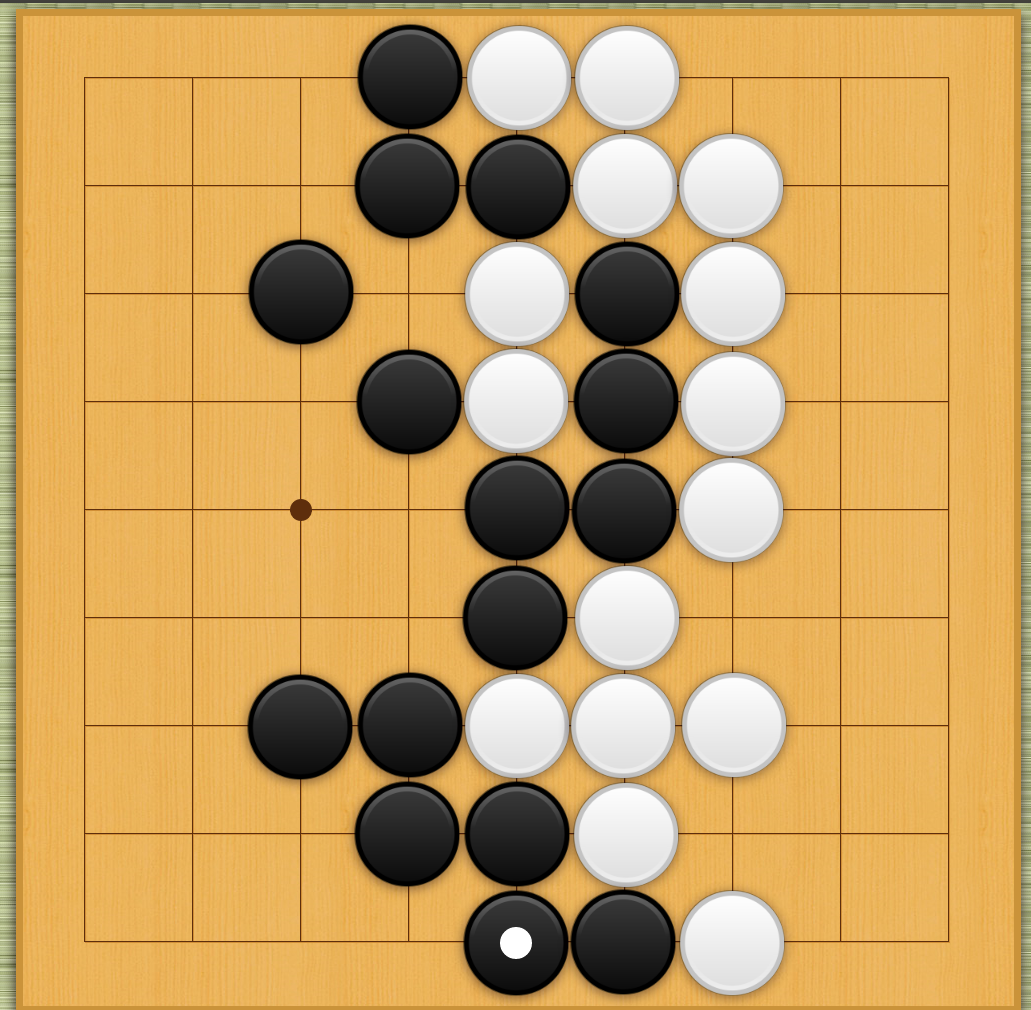
\includegraphics[scale=0.17]{ejemplo-conteo-negroult.png} \ \ \ Blanco: 21 \ \ \ Negro : 33  
  
  Diferencia: 12
  
\end{frame}

\begin{frame}{Ejemplo conteo de área}
  
    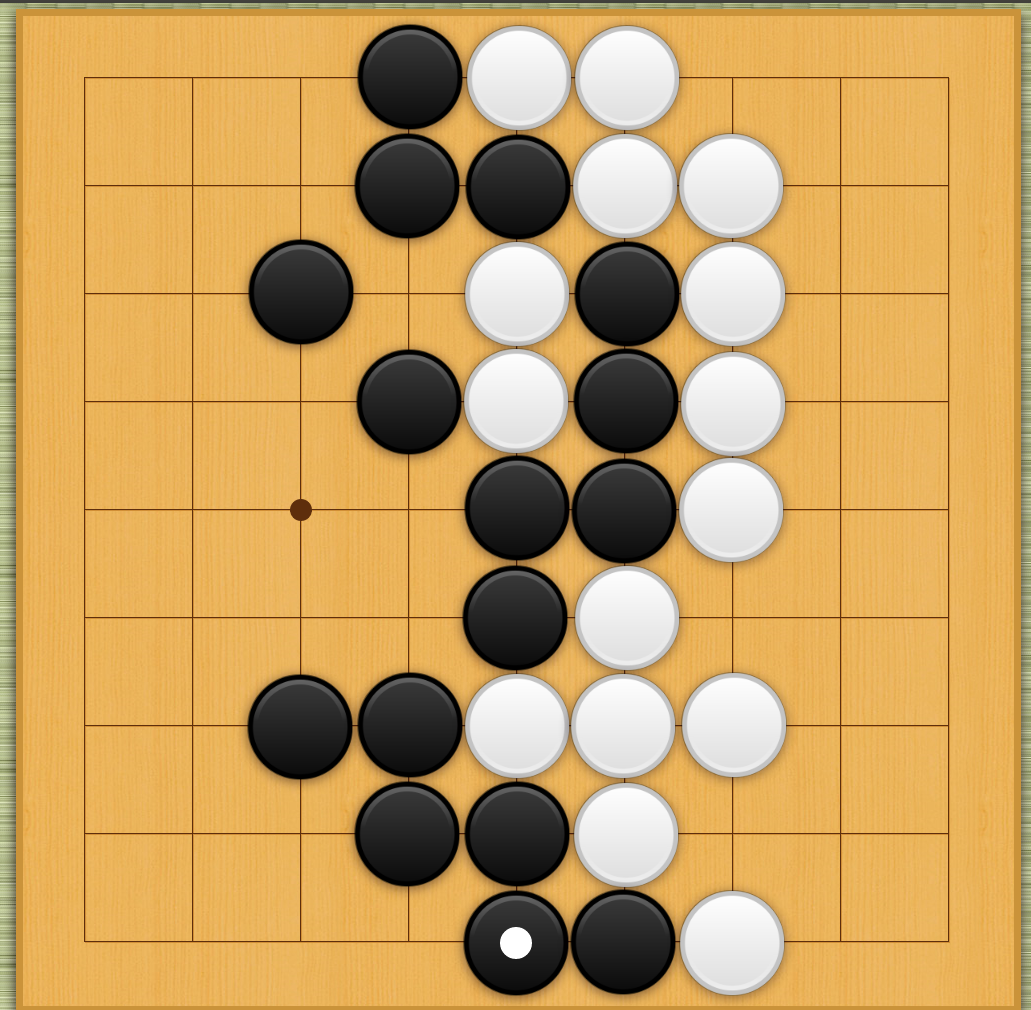
\includegraphics[scale=0.17]{ejemplo-conteo-negroult.png} \ \ \ Blanco: 34 \ \ \ Negro : 47  
  
  Diferencia: 13
  
\end{frame}

\begin{frame}{Recapitulando}

    \begin{itemize}
        \item Conteo de área da el mismo resultado que conteo de territorio, ``redondeado'' en favor de negro a la paridad correcta.
        \item Cualquier diferencia en el conteo mayor a este redondeo es por:
           \begin{itemize}
              \item Pasadas extra (un jugador pasa y el otro no)
              \item Casos donde una intersección es territorio en reglas chinas pero no en reglas japonesas y viceversa (las veremos)
           \end{itemize}
        \item En reglas con conteo de área, es especialmente importante no pasar si quedan dames pues podemos perder puntos.
    \end{itemize}
  
\end{frame}

\begin{frame}{Conteo AGA}

    \begin{itemize}
        \item \textbf{Las reglas AGA utilizan conteo de área.}
        \item Se suele decir que las reglas AGA ``reconcilian'' área y territorio usando passing-stones, pero eso es solo un truco de conteo que permite
          calcular el área (``puntaje chino'') contando con el método tradicional japonés. El puntaje de las reglas AGA resulta ser como en reglas chinas.
        \item Passing Stones: 
          \begin{itemize}
             \item Cada vez que un jugador pasa, da una piedra prisionera a su rival.
             \item Si negro pasa por última vez, blanco le da una piedra más.
          \end{itemize}
        \item Siempre vale que al usar passing stones y contar territorio, se obtiene la misma diferencia exacta que si se hubiera contado área directamente.
    \end{itemize}
  
\end{frame}

\begin{frame}{Mitos}

    \begin{itemize}
        \item ``Conteo de área es más laxo (es inofensivo defender de más)''
          \begin{itemize}
             \item Falso: mientras uno defiende, el rival llena dames, que valen un punto. Jugar en territorio propio entonces pierde puntos mientras quedan dames.
          \end{itemize}
        \item ``Reglas chinas = conteo de área, \\Reglas japonesas = conteo de territorio''
          \begin{itemize}
             \item Falso: hay otras diferencias que son \textbf{más importantes}, pues como vimos esto solo cambia un puntito en condiciones normales.
          \end{itemize}
        \item ``Las reglas de territorio son formalmente más complicadas''
          \begin{itemize}
             \item Falso: hay reglas con conteo de territorio formalmente simples (pero no son de uso común). La complejidad formal de las reglas japonesas está en otra parte, no en el conteo de territorio.
          \end{itemize}
    \end{itemize}
  
\end{frame}

\begin{frame}{Dames unilaterales}

    \begin{itemize}
        \item A veces pueden existir dames que solamente puede llenar un jugador.
        \item Las reglas japonesas no dan puntos por ellos, a pesar de que se comportan como cualquier otro territorio seguro de un jugador.
        \item En reglas chinas / AGA, se puede esperar al final del juego, una vez terminado y llenados todos los dames, para llenar estos puntos y poder contarlos como territorio.
        \item Por esta razón, las reglas chinas y AGA cuentan los dames unilaterales como territorio, mientras que las japonesas no.
    \end{itemize}
  
    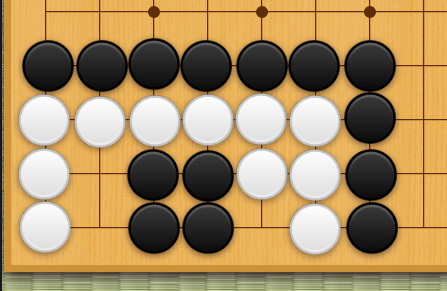
\includegraphics[scale=0.3]{unilateral.png} Negro tiene un punto de territorio
  
\end{frame}

\begin{frame}{Puntos de grupos en seki}

    \begin{itemize}
        \item Reglas japonesas hacen una distinción para seki
        \item No hay territorio ni prisioneros en un seki
        \item En reglas chinas y AGA, se cuentan los puntos
        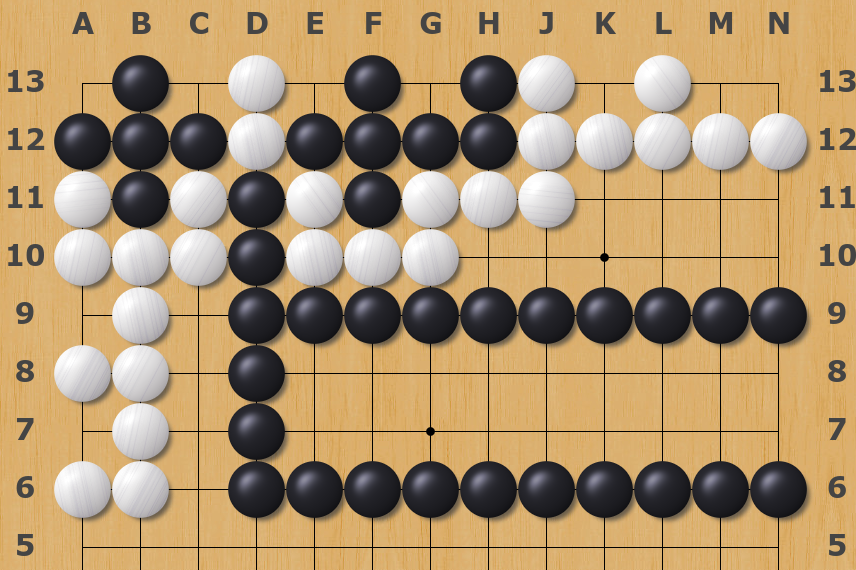
\includegraphics[scale=0.25]{sekisinpuntos.png}
    \end{itemize}
  
\end{frame}


\section{Fin del juego}

\begin{frame}{Condición de terminación}

    \begin{itemize}
        \item Difícil para los principiantes determinar cuándo termina el juego
        \item Intuición: ``Cuando todos los territorios están delimitados, y no hay nada más por hacer''
        \item Problema: situaciones de ko extrañas
        \item Por practicidad las reglas más habituales son:
          \begin{itemize}
              \item El juego termina cuando los dos jugadores pasan consecutivamente (Reglas japonesas, AGA). 
              \item El juego termina cuando los dos jugadores acuerdan que terminó (Reglas chinas, según la traducción que encontré). 
          \end{itemize}
    \end{itemize}
  
\end{frame}

\begin{frame}{Punto del último ko}

    \begin{itemize}
        \item Supongamos que queda un último ko, y ya no hay más dames ni nada para llenar.
        
    \end{itemize}
    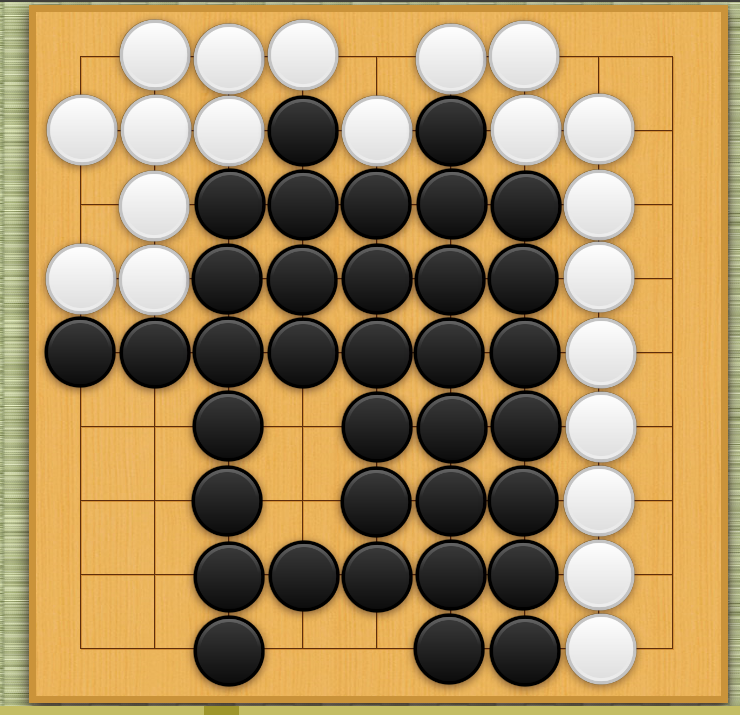
\includegraphics[scale=0.2]{last-ko.png} ¿Qué pasa con el ko? 
  
\end{frame}

\begin{frame}{Punto del último ko (cont)}

    \begin{itemize}
        \item Las reglas chinas, AGA y similares con conteo de área permiten a blanco quedarse con ese punto: para eso no tiene más que llenar el punto del ko
         normalmente, pues como ya no queda nada más en el tablero (ni dames), llenar para asegurarlo es gratuito, y el resultado será el mismo que si hubiera pasado
         teniendo ese punto de territorio.
        \item Las reglas japonesas, si bien durante un tiempo permitieron quedarse con ese punto de territorio, desde 1949 en sus formas escritas prohíben
         quedarse con ese punto de territorio: blanco está obligado a defender el ko, no importa cuántas amenazas de ko tenga
    \end{itemize}
  
\end{frame}

\begin{frame}{Luchas de ko llenando dames}
  \begin{itemize}
   \item Si hay dames libres, llenar el ko no es gratis, y en reglas chinas es por eso que llenar el ko cuando ya no quedan dames es un punto más valioso que llenarlo
          antes, pues corresponde a ganar el ko y además quedarse con ese punto de territorio.
        \item Esto mismo pasaría en reglas japonesas si permitieran quedarse con ese punto de territorio: sería más valioso seguir luchando el ko hasta agotar los dames,
        para poder pasar al final y guardarse ese territorio sin tener que defender el ko. Como las reglas japonesas modernas prohíben quedarse con ese punto, tal lucha de ko
        usando dames carece de sentido.
  \end{itemize}
\end{frame}

\section{Vida y muerte}

\begin{frame}{Grupo vivo en reglas chinas y AGA}
    \begin{itemize}
        \item Al final, se sacan los grupos muertos para el conteo.
        \item \textbf{¿Qué es un grupo muerto?}
        \item En reglas AGA y Chinas, los jugadores se ponen de acuerdo para contar en cuáles grupos están muertos.
        \item Si no hay acuerdo, entonces se sigue jugando desde la posición que quedaba. Cuando vuelvan a pasar dos veces consecutivas, \textbf{todo lo que quedó en el tablero está vivo}.
        \item \textbf{Vida global}: se juega en todo el tablero, y amenazas de ko lejanas pueden cambiar el status.
    \end{itemize}
    
\end{frame}

\begin{frame}{Grupo vivo en reglas japonesas}
    \begin{itemize}
        \item En reglas japonesas, para saber si un grupo está vivo o muerto, se aplica el \textbf{juego hipotético}.
        \item En juego hipotético, \textbf{no quedan amenazas de ko} (así se explica el bent four): La única opción posible para liberar una prohibición de tomar el ko, es decir "paso".
        \item Un grupo de un jugador está vivo si se da la siguiente condición:
            \begin{itemize}
                \item Existe en juego hipotético una estrategia para el jugador que asegura que, haga lo que haga su rival, nunca será capturado o, si el grupo es capturado, entonces
                 el jugador logra ubicar \textbf{una nueva piedra permanente en la localidad del grupo}. 
            \end{itemize}
    \end{itemize}
    
\end{frame}

\begin{frame}{Grupo vivo en reglas japonesas (cont.)}
    \begin{itemize}
        \item La vida de cada grupo se analiza independientemente.
        \item Únicamente se retiran como prisioneros los grupos muertos que están dentro de territorio (no seki) del rival.
        \item La definición formal y precisa de localía es compleja [Por ejemplo, modelo Jasiek 2003].
        \item La noción de vida es \textbf{local}: La situación de amenazas de ko lejanas no son relevantes.
    \end{itemize}
    
\end{frame}

\begin{frame}{Ejemplo 1: Incapturable}
    Los grupos negros son incapturables: haga lo que haga el rival, no hay estrategia que le permita capturarlos en juego hipotético.
    
    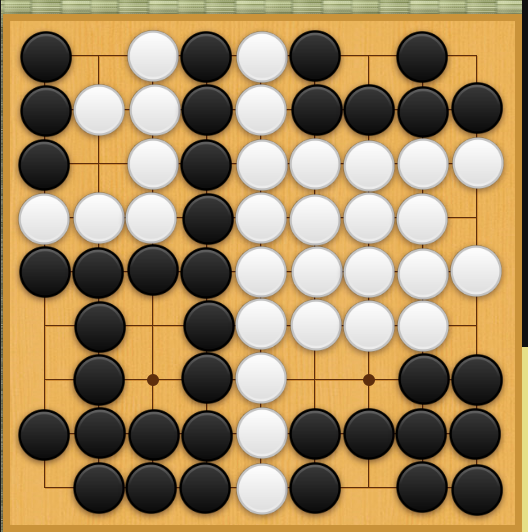
\includegraphics[scale=0.3]{incapturable.png}
    
\end{frame}

\begin{frame}{Ejemplo 1: Blanco es capturable y muere completamente}
    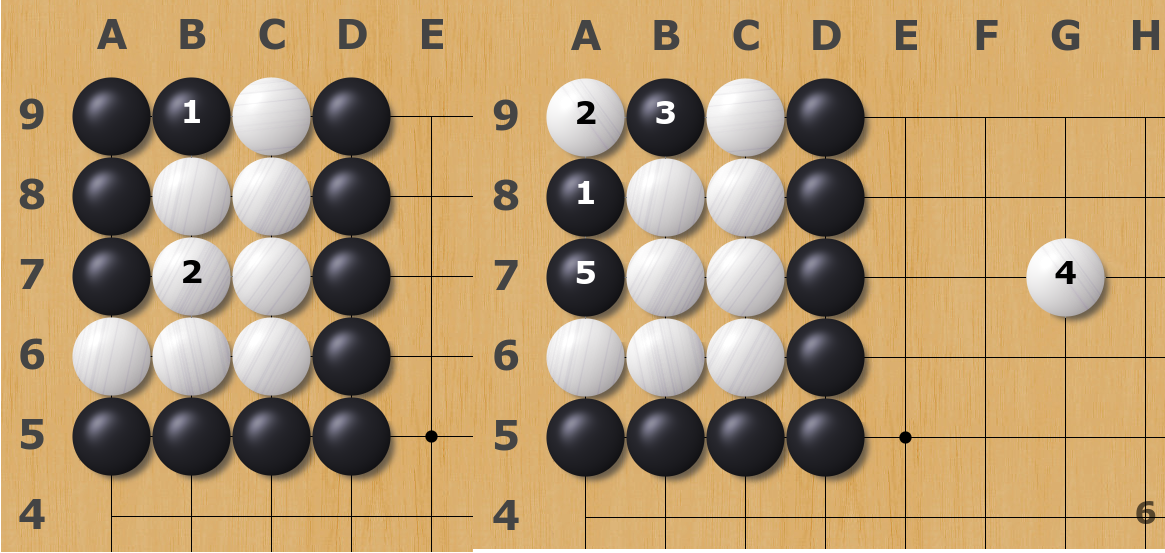
\includegraphics[scale=0.27]{bent4.png}
    
\end{frame}

\begin{frame}{Ejemplo 2: Capturable, localidad directa}
    El grupo de dos piedras negras está vivo (y las piedras blancas, muertas): son capturables, pero entonces luego negro puede capturar todo y volver a colocar una piedra en donde estaban.
    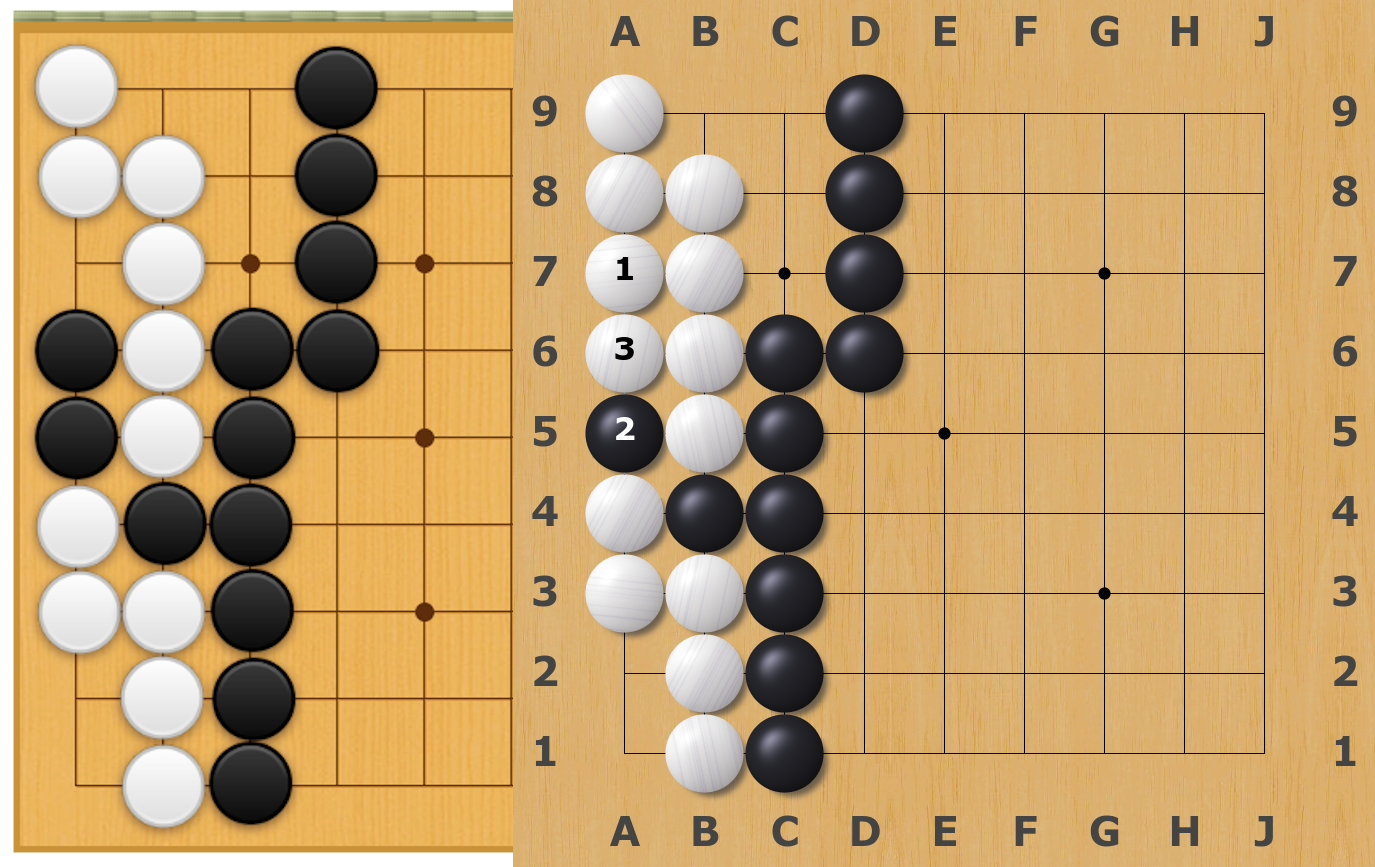
\includegraphics[scale=0.2]{matartodo.png}
\end{frame}

\begin{frame}{Ejemplo 3: Capturable, localidad indirecta}
    Las dos piedras negras de la esquina están vivas (en seki). Si bien blanco puede capturarlas por completo, y negro no podría volver a jugar nada en esa esquina, gracias a esas dos piedras 
     negro podría ubicar \textbf{nuevas piedras permantentes} en las casillas marcadas con cuadrado, si es que blanco se decide efectivamente a capturar las piedras de la esquina. 
     
     Estas posibles
     nuevas piedras permanentes hacen que las originales estén vivas.
    
    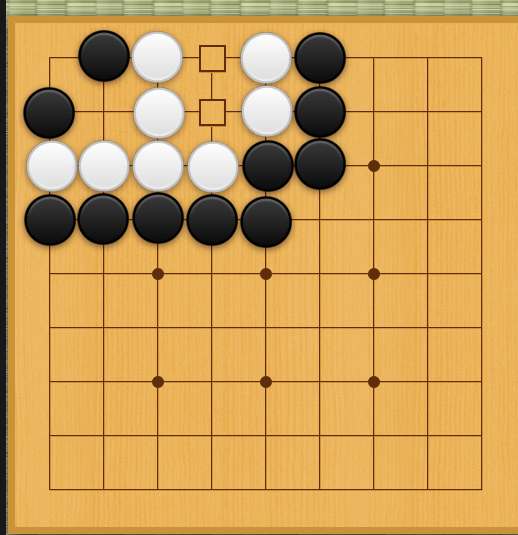
\includegraphics[scale=0.3]{capturable2.png}
\end{frame}

\begin{frame}{Ejemplo 4 (avanzado): Bent four + sekis}
        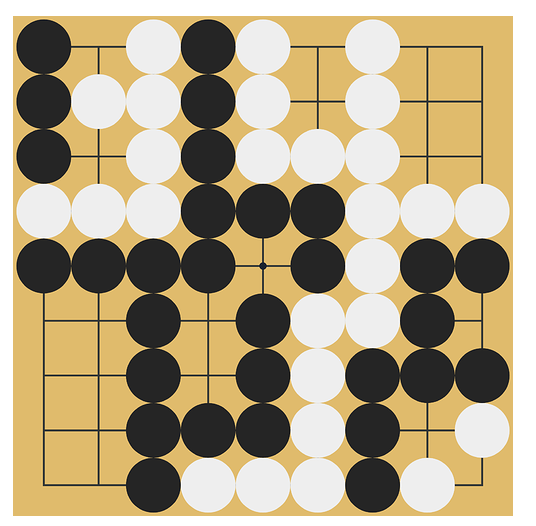
\includegraphics[scale=0.3]{tsumego1.png}
        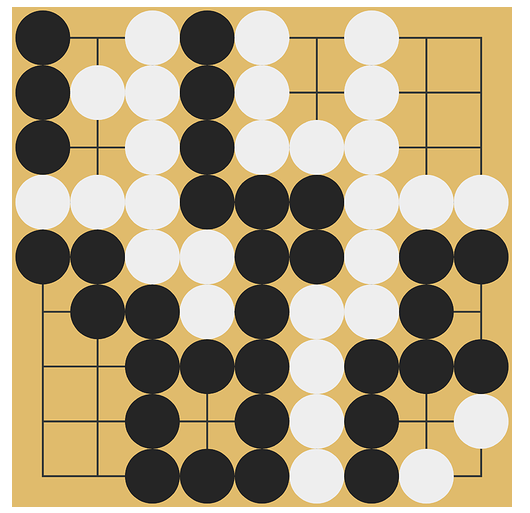
\includegraphics[scale=0.3]{tsumego2.png}
        
        ¿Cuál es el resultado? ¿Depende de las reglas? ¡A Discord! \#reglas
\end{frame}


\begin{frame}{Seki}
    \begin{itemize}
        \item Las reglas chinas y AGA no definen Seki, y no lo necesitan pues no hacen ninguna distinción entre un grupo vivo con 2 ojos o un grupo en seki.
        \item Las reglas japonesas 1989 definen un grupo en Seki, como un grupo que sigue adyacente a un dame al terminar el juego.
    \end{itemize}
    La definición utilizada en las reglas japonesas 1989 tiene el defecto de permitir ``pseudosekis''.
    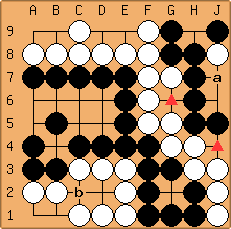
\includegraphics[scale=0.4]{pseudoseki.png}
    \\
    Preguntar en Discord en \#reglas :)
\end{frame}

%\begin{frame}{Torazu Sanmoku}
%    \begin{itemize}
%        \item Esta posición fue cambiada por las reglas 1989 (y por las del WAGC)
%    \end{itemize}
%    
%    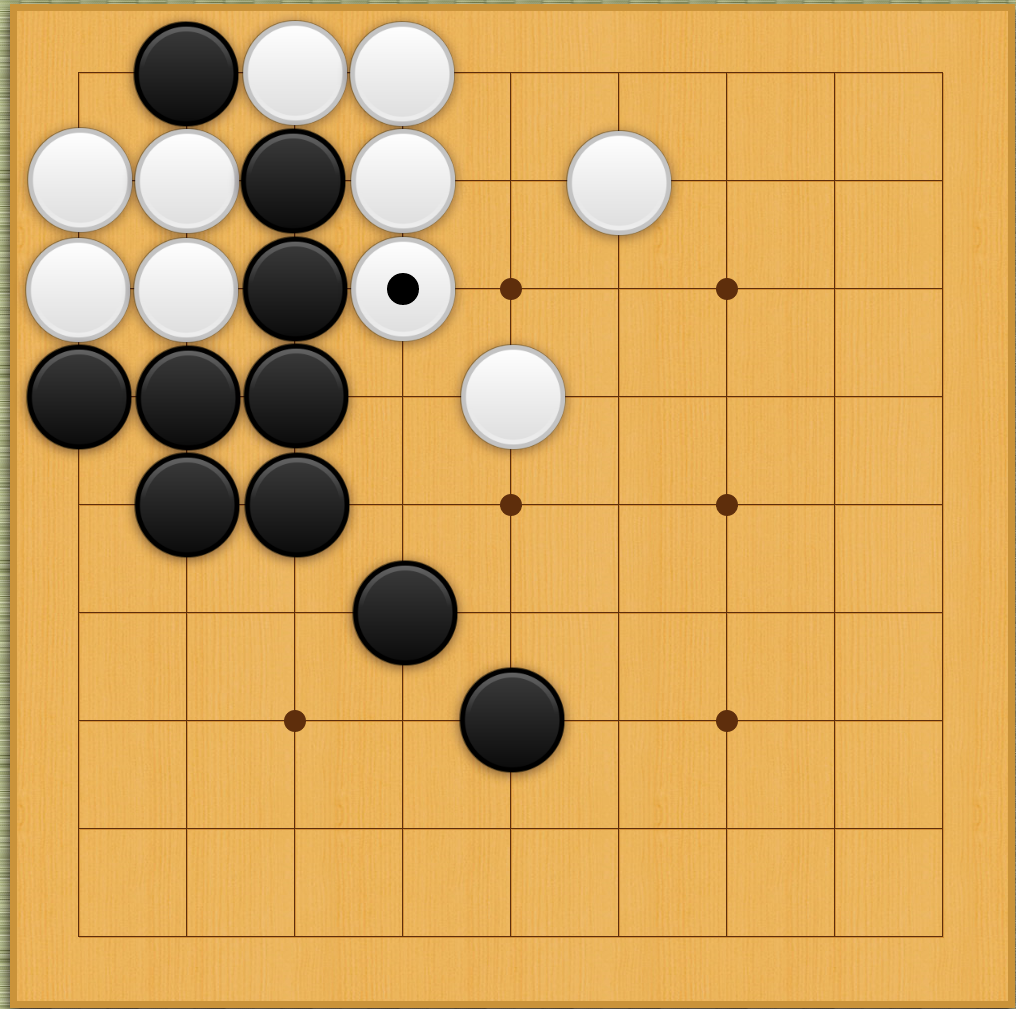
\includegraphics[scale=0.2]{torazu-sanmoku.png}
%\end{frame}
%
%\begin{frame}{Torazu Sanmoku (cont.)}
%    \begin{itemize}
%        \item Cuando fue consultado por esta posición, shuwa determinó que negro tenía 3 puntos, sin necesidad de jugar.
%            \begin{itemize}
%              \item Es decir, lo evaluó como si fuera un caso de snapback típico.
%              \item Si empieza capturando blanco (snapback), negro puede conseguir 3 puntos.
%              \item Si empieza capturando negro en cambio, solo puede conseguir 2 puntos.
%            \end{itemize}
%        \item El procedimiento de vida y muerte actual determina que la situación es 0 puntos (seki, ambos vivos) si queda en el tablero.
%        \item Por lo tanto, actualmente lo que debe hacer negro es capturar, y aceptar quedarse con solo 2 puntos.
%    \end{itemize}
%\end{frame}


\begin{frame}{Falsa vida}
    Es una situación que todas las reglas principales determinan como muerta, pero que generó disputas durante cientos de años.
    
    Se produce esta situación cuando es imposible capturar un ``ko muerto'', que por sí solo no podría vivir, ya que el rival cuenta con infinitas amenazas de ko. 
    
    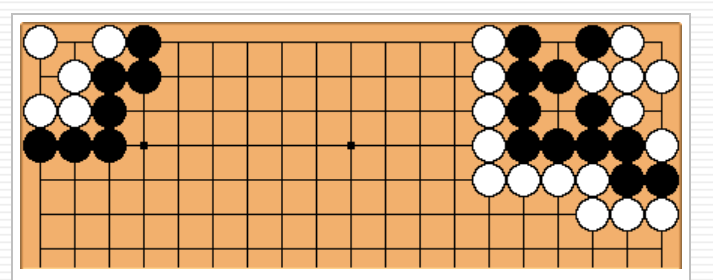
\includegraphics[scale=0.4]{falsa-vida.png}
\end{frame}

\begin{frame}{Falsa vida (cont.)}
    Un grupo de estas características está muerto con las 3 reglas principales porque:
    \begin{itemize}
        \item Las reglas AGA utilizan superko, y en ese caso el grupo no logra evitar ser capturado, pues la regla del ko le impide seguir recapturando.
        \item En reglas japonesas se utiliza el juego hipotético, y entonces la localidad de la vida y muerte hace que las infinitas amenazas de ko no se puedan utilizar.
    \end{itemize}
\end{frame}

\begin{frame}{Falsa vida (cont.)}
    Las reglas chinas también utilizan superko peeeero:
    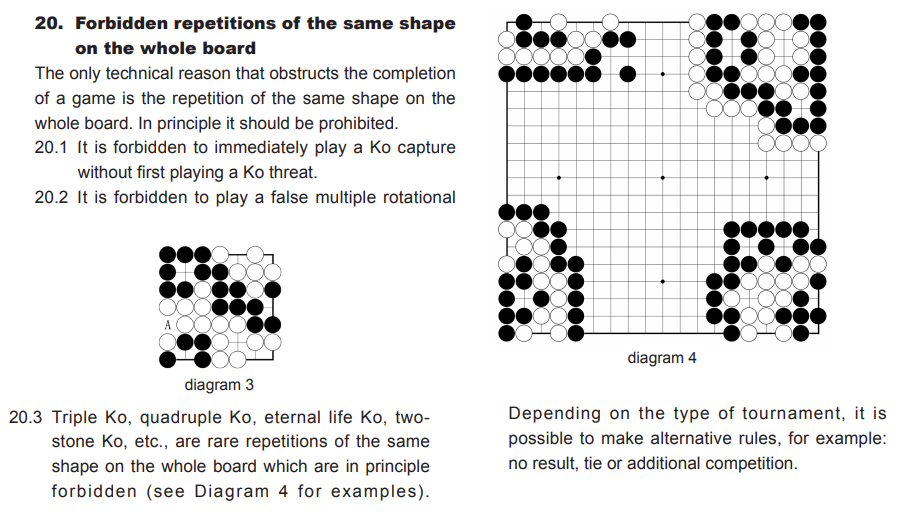
\includegraphics[scale=0.39]{chinesesuperko.png}
\end{frame}

\section{Ko (repetición)}

\begin{frame}{Triples ko (y similares repeticiones) famosos}
  
  Las siguientes partidas terminaron sin resultado, por triple ko:
  
  \begin{itemize}
    \item 1582: Honinbo Sansa vs Kashio Rigen
       \begin{itemize}
         \item Ante Oda Nobugana en Tokyo. Al día siguiente es asesinado.
         \item Desde entonces se consideró triple ko $=$ mala suerte.
       \end{itemize}
    \item 1998: O Rissei vs Cho Chikun (Cuarto juego del título Meijin)
  \end{itemize}
  
  El siguiente pudo terminar en triple ko, pero Luo eligió ceder el triple ko a su rival, y aún así ganó el partido.
  
  \begin{itemize}
     \item 2005: Luo Xihe vs Choi Cheolhan (Semifinales de Copa Samsung)
  \end{itemize}
  
  El siguiente partido terminó sin resultado, por \textbf{cuádruple ko}:
  
  \begin{itemize}
     \item 2007: Kono Rin vs Akiyama Jiro (Copa Agon)
  \end{itemize}
  
  ``Of the 168 813 games played by Nihon Kiin professionals in this period, only 19 have yielded no result, averaging about 1 no result game every 9000 played.''
  
  
  
\end{frame}

\begin{frame}{Triples ko}
    Consisten de 3 ko que los jugadores luchan a la vez:
    
    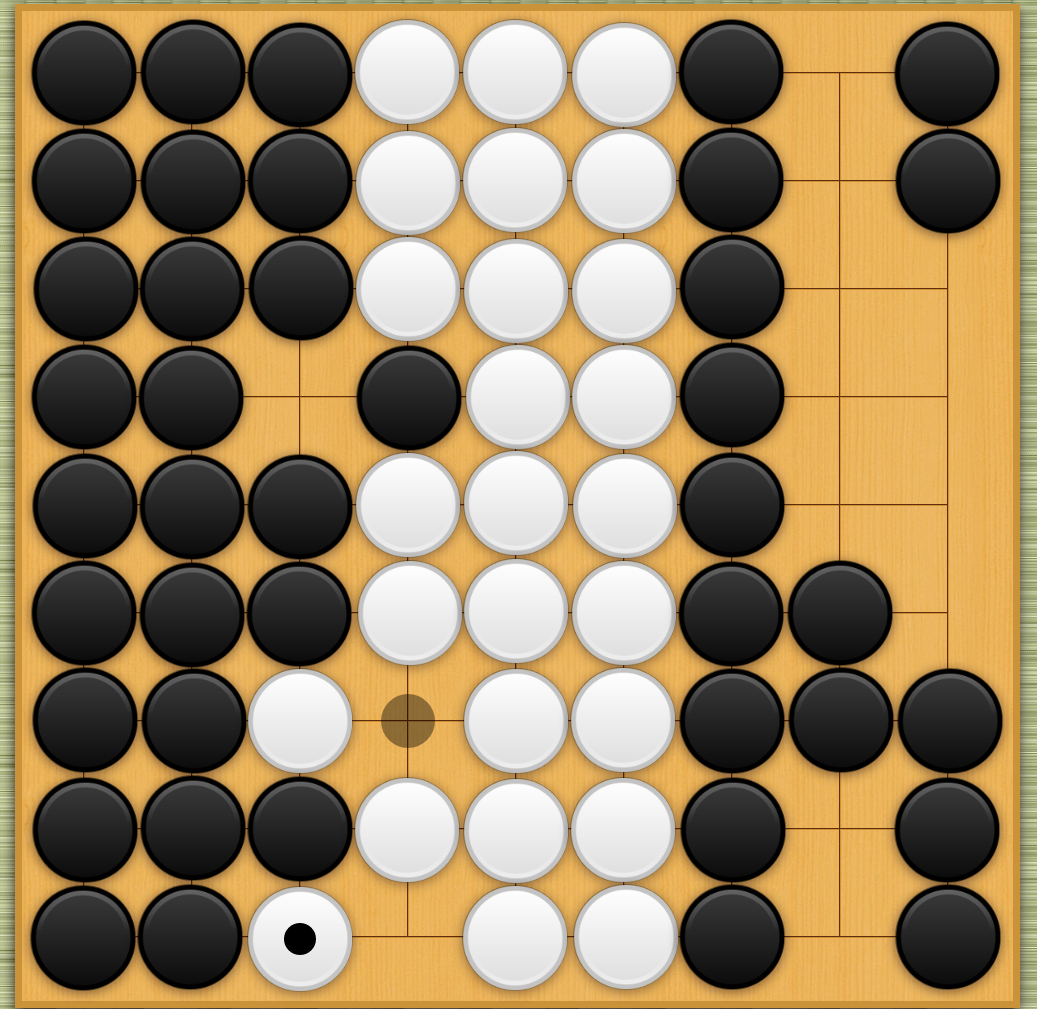
\includegraphics[scale=0.2]{triple-ko.png}
    
\end{frame}

\begin{frame}{Vida eterna}
    Es una configuración extremadamente rara. Aparentemente un texto chino sobre Go diría que si esta situación ocurre:
    
    \begin{itemize}
        \item ``Deberías comprar pescado, verduras, carne y vino, y hacer una buena fiesta para celebrar.''
    \end{itemize}
    
    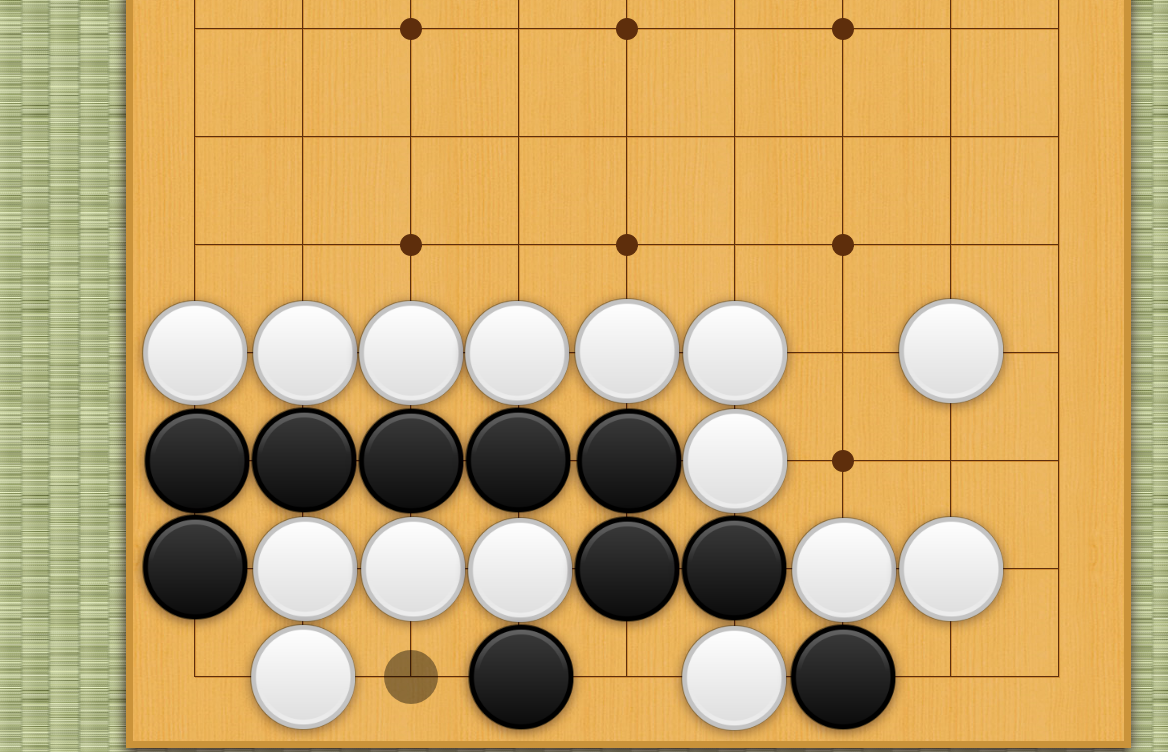
\includegraphics[scale=0.2]{vida-eterna.png}
    
\end{frame}

\begin{frame}{Triples ko y vida eterna: tratamiento}
    Ante estas secuencias con repeticiones:
    
    \begin{itemize}
        \item Si ninguno de los jugadores cede el ciclo, las reglas japonesas \textbf{anulan el partido}.
        \item Las reglas chinas en la práctica lo dejan a criterio de cada torneo.
        \item Las reglas AGA utilizan superko:
        \begin{itemize}
          \item No se permite repetir \textbf{ninguna} situación del tablero que ya haya ocurrido en algún momento previo.
          \item Según cada posición particular, podría darse una lucha de ko, o quedar un grupo en ``falsa vida''.
        \end{itemize}
        
    \end{itemize}
\end{frame}

\section{Resumen de reglas ``Convencionales''}

\begin{frame}{Chinas}
    \begin{itemize}
        \item Conteo de área
        \item Superko en teoría, pero a veces permiten anular por triple ko.
        \item Vida y muerte global: Se juega, y todo lo que queda en el tablero está vivo.
        \item Seki es territorio, no hace diferencia.
    \end{itemize}
\end{frame}

\begin{frame}{Japonesas}
    \begin{itemize}
        \item Conteo de territorio
        \item Solo la regla de ko básica
        \item Vida y muerte local, con juego hipotético y sin amenazas de ko
        \item Seki NO es territorio.
    \end{itemize}
\end{frame}

\begin{frame}{AGA}
    \begin{itemize}
        \item Conteo de área
        \item Superko situacional
        \item Vida y muerte global: Se juega, y todo lo que queda en el tablero está vivo.
        \item Seki es territorio, no hace diferencia.
    \end{itemize}
\end{frame}


\section{Reglas ``No convencionales''}

%\begin{frame}{Suicidio}
%    \begin{itemize}
%        \item Las reglas más usadas no permiten suicidio, pero otras sí.
%        \item Notoriamente, en Taiwan y algunos torneos europeos se utilizan las reglas Ing (o Ing simplificadas), que sí lo permiten.
%    \end{itemize}
%\end{frame}
%
%\begin{frame}{Ejemplo de suicidio útil más común}
%    A veces, luego de un oshi-tsubushi, queda una jugada posible de suicidio, que puede utilizarse como \textbf{amenaza de ko adicional}.
% 
%    {\hfill 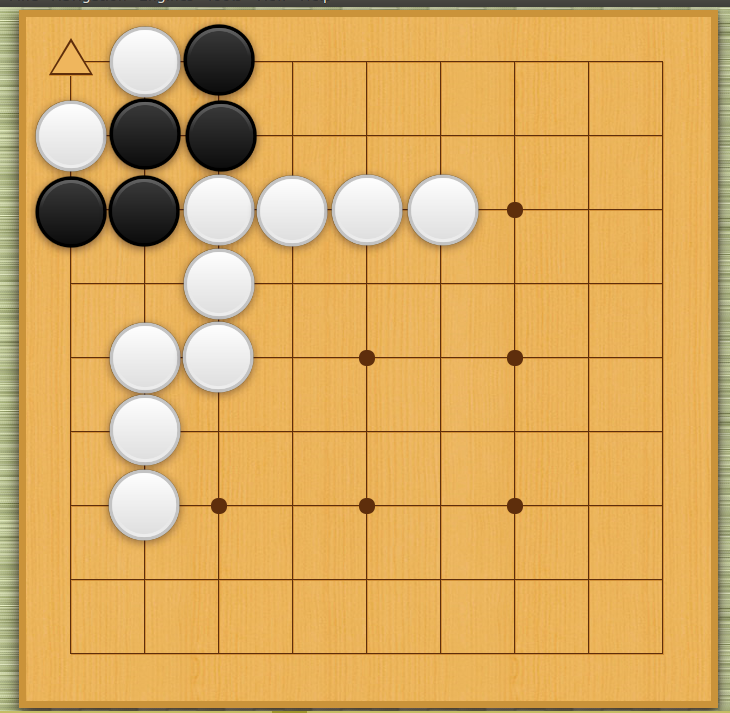
\includegraphics[scale=0.25]{suicidio-amenaza.png} \hfill}
%\end{frame}
%
%\begin{frame}{Ejemplo de suicidio útil más raro}
%\vspace{-1.5cm}
%    Un ejemplo mucho menos frecuente donde el suicidio es útil, pero más espectacular, es en algunas carreras de capturar. De alguna manera, el suicidio permite ``corregir una muy mala forma''.
%    
% \begin{wrapfigure}{L}{0.52\linewidth}
%    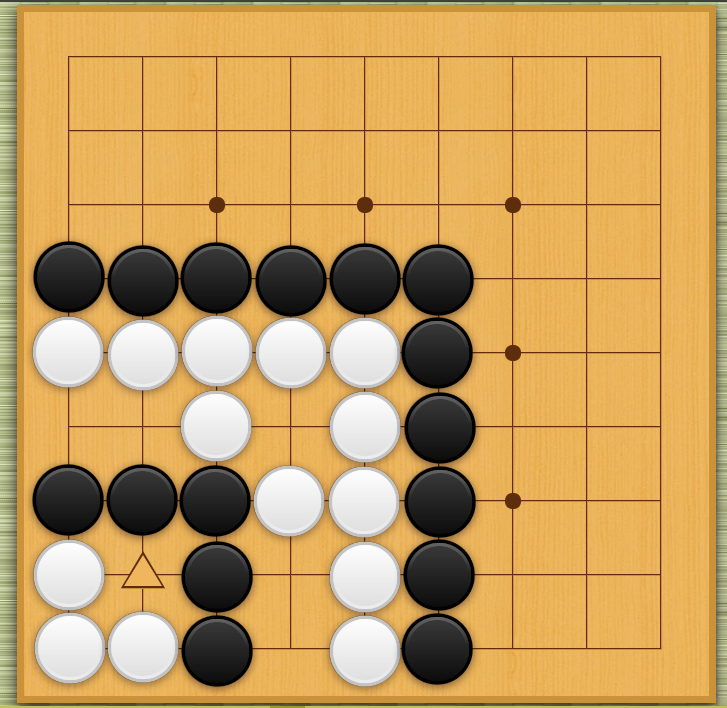
\includegraphics[scale=0.25]{suicidio-carrera.png} 
%\end{wrapfigure}
%
%\vspace{-0.4cm}
%
%\ 
%
%\ 
%
%En la posición que se muestra a la izquierda, si no hay suicidio, blanco muere inevitablemente. 
%
%\ 
%
%Pero si en cambio se permite el suicidio y blanco juega en el triángulo, puede crear un seki.
%
%\end{frame}


\begin{frame}{Sunjang Baduk}
    \begin{itemize}
        \item Forma de go común en Corea entre los siglos XVI y XX.
        \item Piedras iniciales preubicadas en un patrón ``de lucha'' fijo. 
        \item Sistema de conteo no convencional: al terminar se sacan piedras internas dejando solo las ``fronteras'' de los territorios, y se cuenta el territorio interno, ignorando prisioneros.
    \end{itemize}
    
    {\hfill 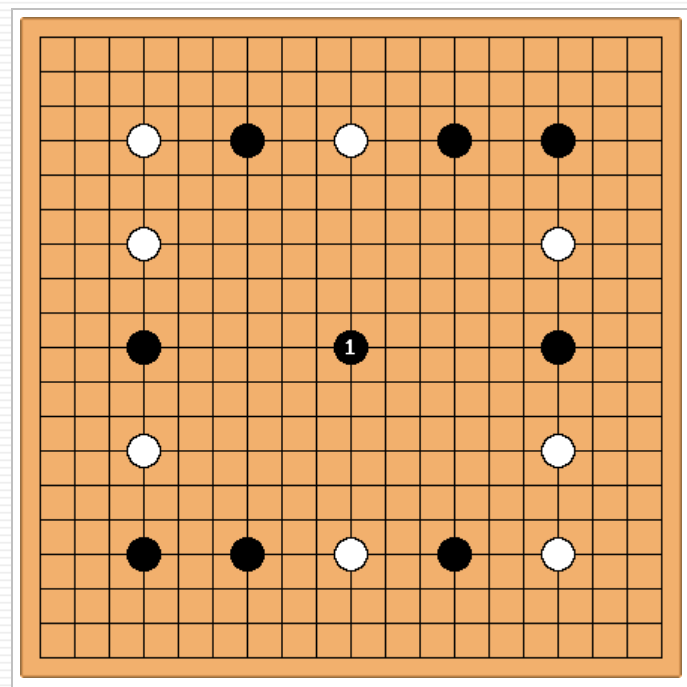
\includegraphics[scale=0.2]{sunjang-baduk.png} \hfill}
    
\end{frame}

\begin{frame}{Go tibetano}
\footnotesize
    \begin{itemize}
        \item Tablero de 17x17
        \item Blanco juega primero (lo mismo ocurría en la antigua China)
        \item Piedras iniciales preubicadas en un patrón ``de lucha'' fijo.
        \item Regla del ko modificada: 
            \begin{itemize}
            \footnotesize
              \item ``No se puede jugar una piedra en una intersección de la cual el oponente acaba de retirar una piedra capturada''
              \item Esto además de prohibir la recaptura de ko usual, también prohíbe el snapback inmediato: para recapturar un ``snapback'' hay que gastar una amenaza de ko.
            \end{itemize}
    \end{itemize}
    
    \vspace{-0.1cm}
    {\hfill 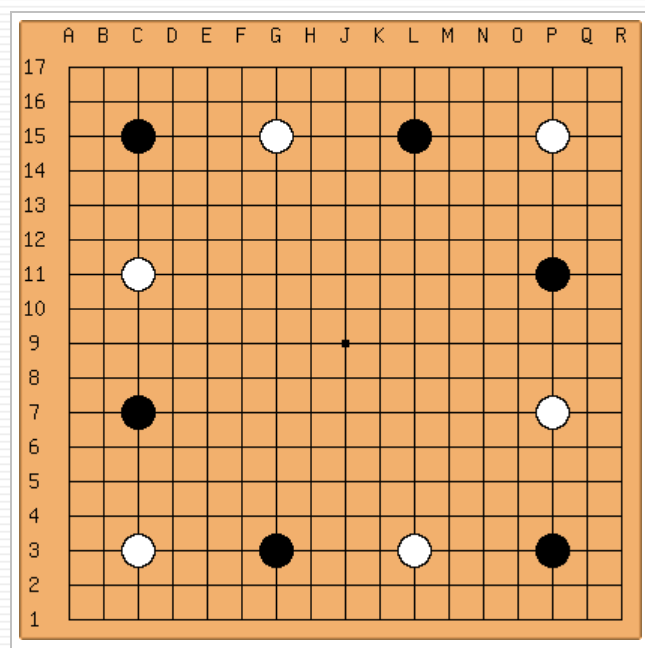
\includegraphics[scale=0.17]{go-tibetano.png} \hfill}
    
\end{frame}


\section{Lecturas recomendadas}

\begin{frame}{Bibliografía}

    \begin{itemize}
        \item \url{https://senseis.xmp.net/?RulesOfGo}
        \item \url{https://senseis.xmp.net/?GoRulesBestiary}
        \item \url{http://harryfearnley.com/go/bestiary/rule_challenge.html}
        \item \url{http://elsantodel90.tk/go-rules/go-rules.html}
        \item \url{https://groups.google.com/forum/\#!topic/rec.games.go/WgKwxzN61g4}
        \item \url{https://senseis.xmp.net/?SendingTwoReturningOne}
        \item \url{https://forums.online-go.com/t/odd-cases-in-the-japanese-rules}
        \item \url{https://web.archive.org/web/20130112213532/http://www.gogod.co.uk/NewInGo/C\%26IP.htm}
    \end{itemize}

\end{frame}


\end{document}
